\section{Unit Analysis}
We will now take a look at three Terran units which could be interesting to micro. In the analysis of the units we will
focus on the range, movement speed, damage, armor, availability, micro benefits, and fire cooldown. 

\subsection{Marines}
\begin{table}[H]
	\begin{tabular}{| l | c | c}
		\cline{1-2}	
		Hit points		& 40		&\multirow{5}{*}{
\includegraphics[scale=.4]
									{Figures/Units/marine.png}} \\ \cline{1-2}
		Range			& 4 		&\\ \cline{1-2}
		Weapon Cooldown	& 7.5/15 	&\\ \cline{1-2}
		Price			& 50m		&\\ \cline{1-2}
		Building needed	& Barracks	&\\ \cline{1-2}
	\end{tabular}
\end{table}

Marines are interesting because they can shoot air and ground units. The upgrade \textit{stimpacks} increases the marines movement speed and doubles the fire rate. This makes the unit very dynamic and gives it high micro benefits. Marines are easy to get and are normally the first unit a Terran uses in
their army. Marines only have a range of 4 and are the slowest unit that we are going to take a look at. Their hit points are only 40. Since marines can be gotten so early, they are a good candidate for the project. On the other hand, to get the full benefit from the marines they need upgrades and support from medics to heal them. 

\subsection{Vultures}

\begin{table}[H]
	\begin{tabular}{| l | c | c}
		\cline{1-2}
		Hit points		& 80		&\multirow{5}{*}{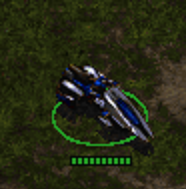
\includegraphics[scale=.4]
									{Figures/Units/vulture.png}}	\\ \cline{1-2}
		Range			& 5 		&\\ \cline{1-2}
		Weapon Cooldown	& 30 		&\\ \cline{1-2}
		Price			& 75m		&\\ \cline{1-2}
		Building needed	& Factory	&\\ \cline{1-2}
	\end{tabular}
\end{table}

Vultures are a little car with a high speed. Because of a longer range the vulture can out range the marine. Like the marines, the
vultures also have upgrades. The most interesting upgrade is the spider mines that allows the vultures to place three mines. When another unit goes near the mine it will detonate dealing a large amount of splash damage. The vultures are made
from the Factory which means you will be able to get marines before you get vultures. The good thing about vultures is the price is only 75 minerals. Having all this in mind, it is clear that vultures have much to offer in terms of micro.
That being said the vultures fire cooldown is 30 which is twice the marine's cooldown (see reference \cite{wiki_vulture}).

\subsection{Wraiths}
\begin{table}[H]
	\begin{tabular}{| l | c | c}
		\cline{1-2}
		Hit points		& 120		&\multirow{5}{*}{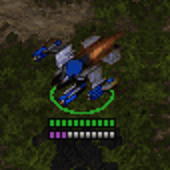
\includegraphics[scale=.4]
									{Figures/Units/wraith.png}}	\\ \cline{1-2}
		Range			& 5 		&\\ \cline{1-2}
		Weapon Cooldown	& 22/30	 	&\\ \cline{1-2}
		Price			& 150m 100g	&\\ \cline{1-2}
		Building needed	& Starport	&\\ \cline{1-2}
	\end{tabular}
\end{table}
Wraiths are air units that can attack ground and other air units. This means that they can move over edges and cliffs which allows it
to move over large distances within a short time period. They are interesting because they have an upgrade that allows them to turn invisible while they have energy. It has the same fire cooldown
as a vulture when attacking ground units and 22 fps when attacking air units.  
The down side of the wraiths is the price (150 minerals and 100 gas) and we need a Starport to built it. This means
there is a long time before you can get actually buy wraith. It is clear there is a lot of micro benefits from choosing this unit. 


%\subsection{Choice of unit}
%As said before the vultures, with its fast speed and long range, could be a interesting unit to choose because the vulture can out micro many types of
%units. It will be easy to deal a lot of damage with the use of multiple attacks and the fast movement speed making it a very dynamic unit. Also the vulture
%is not dependent on other support units like medic. If the vulture is low on health, it can just return back to the base and get repaired. This means
%only one unit type is needed to be controlled. Of cause the down side is the vultures only can attack other ground units like it self. Another down side
%is the slow fire cooldown compared to the marine, but this only means that it will take longer time to kill marines.\\
%If we like to have a fast unit that can fly, like the wraiths, we need to keep in mind that we are very vulnerable in the beginning. This means it is very
%easy for the opponent to win if he scouts our base. Because it is normal to scout in the beginning of the game we are already weakened. So it is clear that
%the wraiths could be a interesting and strong unit to micro, but not as a stand alone unit. We can therefore conclude the best micro unit from the three cases is the vulture.
